\documentclass{beamer}
\usepackage[utf8]{inputenc}

\usepackage{semantic}
\usepackage{graphicx}
\usepackage{booktabs}
%\usepackage{todonotes}
\usepackage[absolute,overlay]{textpos}
\usepackage{tikz}
\usetikzlibrary{decorations.pathmorphing}
\usetikzlibrary{matrix,positioning,arrows}

\tikzset{
mymat/.style={
  matrix of math nodes,
  text height=2.5ex,
  text depth=0.75ex,
  text width=3.25ex,
  align=center,
  column sep=-\pgflinewidth
  }
}



\mode<presentation> {
\usetheme{boxes} % When headline is wanted use Dresden theme instead
\usecolortheme{seagull}
\setbeamertemplate{footline}[page number]
\setbeamertemplate{navigation symbols}{}
}

\input{apl.tex}
\newcommand{\kw}[1]{\texttt{#1}}
\newcommand{\A}[2]{[#1]^{#2}}
\newcommand{\V}[2]{\langle#1\rangle^{#2}}
\renewcommand{\S}[2]{\textrm{S}_{#1}(#2)}
\newcommand{\SV}[2]{\textrm{SV}_{#1}(#2)}
\newcommand{\id}[1]{\textit{#1}}

\newcommand{\IOt}{\texttt{\IO}}
\newcommand{\DDt}{\texttt{\DD}}
\newcommand{\ROt}{\texttt{\RO}}
\newcommand{\UAt}{\texttt{\UA}}
\newcommand{\DAt}{\texttt{\DA}}
\newcommand{\LUt}{\texttt{\LU}}
\newcommand{\TRt}{\texttt{\TR}}
\newcommand{\RVt}{\texttt{\RV}}
\newcommand{\POt}{\texttt{\PO}}
\newcommand{\FMt}{\texttt{\FM}}


\newcommand{\lvl}[1]{\langle #1 \rangle}
\newcommand{\push}[2]{[ #1 ] \lvl{#2}}


\makeatletter
\define@key{beamerframe}{c}[true]{% centered
  \beamer@frametopskip=0pt plus 1fill\relax%
  \beamer@framebottomskip=0pt plus 1fill\relax%
  \beamer@frametopskipautobreak=0pt plus .4\paperheight\relax%
  \beamer@framebottomskipautobreak=0pt plus .6\paperheight\relax%
  \def\beamer@initfirstlineunskip{}%
}
\makeatother

%----------------------------------------------------------------------------------------
%	TITLE PAGE
%----------------------------------------------------------------------------------------

\newcommand{\backupbegin}{
   \newcounter{finalframe}
   \setcounter{finalframe}{\value{framenumber}}
}

\newcommand{\backupend}{
   \setcounter{framenumber}{\value{finalframe}}
}

\title[PhD Defence] % bottom of every slide
  {Array abstractions for GPU programming} % title page

\author{\footnotesize{Martin Dybdal} \\ \footnotesize{\texttt{dybber@dybber.dk}}}

\institute {
HIPERFIT \\
DIKU \\
University of Copenhagen
}

\date[9 August 2017]{9 August 2017}

\begin{document}

\begin{frame}[plain]
\titlepage
\end{frame}



\begin{frame}
  \frametitle{Large-scale data processing}

\begin{textblock}{5}(2,2)
  \centering
  \includegraphics[width=\textwidth]{graphics/lsmplot} \\
  \vspace{-1.5mm}
  Computational finance
\end{textblock}

\begin{textblock}{5}(2,9)
  \centering
  \includegraphics[width=\textwidth]{graphics/opencl_nbody}
   \\
  Physics based simulation
\end{textblock}
\begin{textblock}{5}(9,2)
  \centering
\includegraphics[width=\textwidth]{graphics/neuralnet}
 \\
 \vspace{-3.5mm}
 Machine learning
\end{textblock}
\begin{textblock}{6}(8.5,9)
  \centering
\includegraphics[width=0.8333\textwidth]{graphics/molecularmodeling}
\\
 Bioinformatics/Molecular modeling
% (Bio-)Molecular modeling
\end{textblock}
\end{frame}


\begin{frame}[fragile]
  \frametitle{CPU vs. GPU: Performance}

  \begin{textblock}{5}(10,0.5)
  \centering
  \includegraphics[width=\textwidth]{graphics/geforce-gtx-780-ti}
\end{textblock}
\includegraphics[width=\textwidth]{graphics/cpu-vs-gpu-flops}
\end{frame}


\begin{frame}[fragile]
\frametitle{CPU vs. GPU: Architecture}
\includegraphics[width=\textwidth]{graphics/gpu}

GPUs utilize the transistors of the chip for more computing power,
rather than caches and control logic.

\end{frame}


\newcommand{\twolinebeginparen}{\left(\begin{array}{c} \\ \\ \end{array}\right.}
\newcommand{\twolineendparen}{\left.\begin{array}{c} \\ \\ \end{array}\right)}

\begin{frame}[fragile]
\frametitle{Array programming}

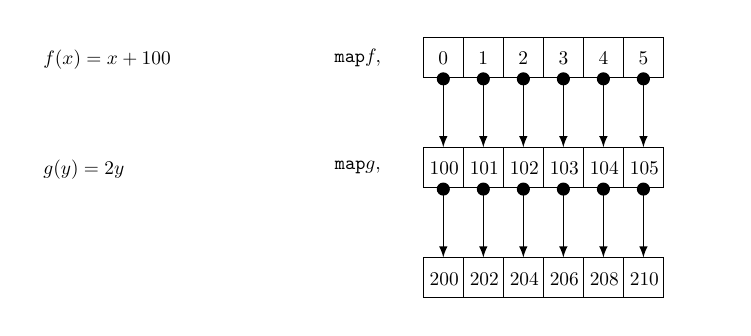
\begin{tikzpicture}[>=latex, scale=0.7, every node/.style={scale=0.7}]
\matrix[mymat, anchor=west,style={nodes=draw}]
at (8,0) 
(mat1)
{
0 & 1 & 2 & 3 & 4 & 5 \\
};

\pause
\matrix[mymat,anchor=west% , style={nodes=draw}
]
at (1,0)
(mat3)
{
f(x) = x + 100 \\
};
\pause

\draw (7,0) node {$\kw{map}\twolinebeginparen f,$};
\draw (13.5,0) node {$\twolineendparen$};

% \matrix [matrix of math nodes,left delimiter={[},right delimiter={]}]
% {
% a_8 & a_1 & a_6 \\
% a_3 & a_5 & a_7 \\
% a_4 & a_9 & a_2 \\
% };

%\pause
%\pause
\matrix[mymat,anchor=west, style={nodes=draw}]
at (8,-2)
(mat2)
{
100 & 101 & 102 & 103 & 104 & 105 \\
};


\begin{scope}[shorten <= -2pt]
\draw[*->]
  (mat1-1-1.south) -- (mat2-1-1.north);
\draw[*->]
  (mat1-1-2.south) -- (mat2-1-2.north);
\draw[*->]
  (mat1-1-3.south) -- (mat2-1-3.north);
\draw[*->]
  (mat1-1-4.south) -- (mat2-1-4.north);
\draw[*->]
  (mat1-1-5.south) -- (mat2-1-5.north);
\draw[*->]
  (mat1-1-6.south) -- (mat2-1-6.north);
% \draw[*->]
%   (mat3-1-1.south) -- (mat2-1-1.north);
% \draw[*->]
%   (mat3-1-1.south) -- (mat2-1-2.north);
% \draw[*->]
%   (mat3-1-1.south) -- (mat2-1-3.north);
% \draw[*->]
%   (mat3-1-1.south) -- (mat2-1-4.north);
% \draw[*->]
%   (mat3-1-1.south) -- (mat2-1-5.north);
% \draw[*->]
%   (mat3-1-1.south) -- (mat2-1-6.north);
\end{scope}



\pause
\matrix[mymat,anchor=west% , style={nodes=draw}
]
at (1,-2)
(mat4)
{
g(y) = 2y \\
};
% \draw (5.65,-2) node {$\times$};

\draw (7,-2) node {$\kw{map}\twolinebeginparen g,$};
\draw (13.5,-2) node {$\twolineendparen$};

\matrix[mymat,anchor=west, style={nodes=draw}]
at (8,-4)
(mat5)
{
200 & 202 & 204 & 206 & 208 & 210 \\
};

\begin{scope}[shorten <= -2pt]
\draw[*->]
  (mat2-1-1.south) -- (mat5-1-1.north);
\draw[*->]
  (mat2-1-2.south) -- (mat5-1-2.north);
\draw[*->]
  (mat2-1-3.south) -- (mat5-1-3.north);
\draw[*->]
  (mat2-1-4.south) -- (mat5-1-4.north);
\draw[*->]
  (mat2-1-5.south) -- (mat5-1-5.north);
\draw[*->]
  (mat2-1-6.south) -- (mat5-1-6.north);
% \draw[*->]
%   (mat4-1-1.south) -- (mat5-1-1.north);
% \draw[*->]
%   (mat4-1-1.south) -- (mat5-1-2.north);
% \draw[*->]
%   (mat4-1-1.south) -- (mat5-1-3.north);
% \draw[*->]
%   (mat4-1-1.south) -- (mat5-1-4.north);
% \draw[*->]
%   (mat4-1-1.south) -- (mat5-1-5.north);
% \draw[*->]
%   (mat4-1-1.south) -- (mat5-1-6.north);
\end{scope}


\end{tikzpicture}


% \begin{textblock*}{0.6\textwidth}(0.1\textwidth,2cm)
% CPU programming
% \begin{verbatim}
% 5+9
%       14
% 14+3
%       17
% 17+22
%       39
% \end{verbatim}
% \end{textblock*}

% \begin{textblock*}{0.7\textwidth}(0.5\textwidth, 2cm)
% GPU programming
% \begin{verbatim}
% (2 4 6 8 10) + 100
%       102 104 106 108 110

% (102 104 106 108 110) * 2
%       204 208 212 216 220
% \end{verbatim}
% \end{textblock*}
\end{frame}

% \begin{frame}[fragile]
% \frametitle{GPU programming}

% Problem:
% \begin{itemize}
% \item GPU cores are bad at ``recalling''
% \item manual control of ``scratch pad''
% \end{itemize}

% \end{frame}

\begin{frame}[fragile]
\frametitle{Fusion}

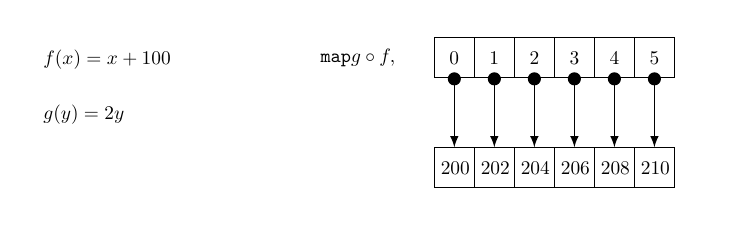
\begin{tikzpicture}[>=latex, scale=0.7, every node/.style={scale=0.7}]
\matrix[mymat, anchor=west,style={nodes=draw}]
at (8.2,0) 
(mat1)
{
0 & 1 & 2 & 3 & 4 & 5 \\
};

\matrix[mymat,anchor=west% , style={nodes=draw}
]
at (1,0)
(mat3)
{
f(x) = x + 100 \\
};


\draw (7,0) node {$\kw{map}\twolinebeginparen g \circ f,$};
\draw (13.5,0) node {$\twolineendparen$};

\matrix[mymat,anchor=west, style={nodes=draw}]
at (8.2,-2)
(mat2)
{
200 & 202 & 204 & 206 & 208 & 210 \\
};


\begin{scope}[shorten <= -2pt]
\draw[*->]
  (mat1-1-1.south) -- (mat2-1-1.north);
\draw[*->]
  (mat1-1-2.south) -- (mat2-1-2.north);
\draw[*->]
  (mat1-1-3.south) -- (mat2-1-3.north);
\draw[*->]
  (mat1-1-4.south) -- (mat2-1-4.north);
\draw[*->]
  (mat1-1-5.south) -- (mat2-1-5.north);
\draw[*->]
  (mat1-1-6.south) -- (mat2-1-6.north);
\end{scope}


\matrix[mymat,anchor=west% , style={nodes=draw}
]
at (1,-1)
(mat4)
{
g(y) = 2y \\
};

\end{tikzpicture}

\pause


$$\kw{map}~g~(\kw{map}~f~array) \equiv \kw{map}~(g \circ f)~array$$



\end{frame}

\begin{frame}
\frametitle{Two projects on array languages}
\begin{itemize}
\item TAIL
  \begin{itemize}
  \item Compiling the array language APL
  \item APL is somewhat widely used in financial industry
  \item Typed functional intermediate language
  \item Several backends
  \end{itemize}
\item FCL
\end{itemize}
\end{frame}

\begin{frame}[plain,c]
%\frametitle{A first slide}
  \begin{center}
    Part I \\
 \huge  TAIL: A Typed Array Intermediate Language for Compiling APL
\end{center}
\end{frame}

%----------------------------------------------------------------------------------------
%	TABLE OF CONTENTS
%----------------------------------------------------------------------------------------

% \begin{frame}
% \frametitle{Overview}
% \tableofcontents
% \end{frame}

%----------------------------------------------------------------------------------------
%	CONTENT
%----------------------------------------------------------------------------------------


\section{Overview}

\begin{frame}
\frametitle{Goals}
\begin{itemize}
\item GPU programming for APL fingers
\item Develop backend technology independently of APL. Other frontends
  could be J, K, some new Haskell vector-library or R-library.
\item Bridging the PL and APL communities
  % \begin{itemize}
  % \item APL compiler writers have been doing fusion since 1970 (at
  %   least), originally they called it ``drag-along''.
  % \end{itemize}
\item Performance on code written by non-programmers (e.g. biologist
  or quant code)
\end{itemize}

\end{frame}


\begin{frame}
\frametitle{Why APL?}
\begin{itemize}
\item 
Notation for non-programmers (biologist/chemist/quants etc.)
\item 
APLs primitives have proven suitable for many applications
\item 
\textbf{APL programs are inherently parallel}
  \begin{quotation}
    \noindent
    "Unlike other languages, the problem in APL is not determining
    where parallelism exists. Rather, it is to decide what to do with
    all of it." \\
      - Robert Bernecky, 1993
  \end{quotation}
\item Existing programs/benchmarks (this is not such a strong point as
  we originally thought)
% \begin{itemize}
% \item We don't have to write our own
% \item Writing the benchmarks ourselves might not represent how it will
%   be used in a production environment
% %\item Writing our own is not always trustworthy. We can specialise
% %  them towards the compiler.
% %\item We want to perform on biologist- and quant-written code.
% \end{itemize}
\end{itemize}

\end{frame}

\begin{frame}
\frametitle{Overview}
\begin{center}
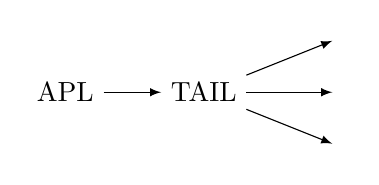
\begin{tikzpicture}[edge from parent/.style={draw,-latex},
                   sibling distance=2em,
                   level distance=5em,
                   every node/.style = {shape=rectangle,
                   align=center}]
  \node {APL}
  child[grow=right] { node {TAIL}
%      child { node { OpenMP } } 
%      child { node { OpenCL } } 
      child { node { } }
      child { node {  } } 
%      child { node { Bohrium } } 
      child { node {  } }
    };
\end{tikzpicture}
\end{center}

\begin{itemize}
\item APL: Dynamically weakly typed array language
\item TAIL: Statically strongly typed array language as target for APL
  and friends.
  \begin{itemize}
  \item type inference
  \item polymorphic shape-types (similar to Repa/Accelerate shapes)
  \item singleton-types
  \item no nested arrays
  \item no heterogeneous arrays
  \end{itemize}
\end{itemize}

\end{frame}


\begin{frame}[fragile]
\frametitle{Brief APL introduction}


\begin{verbatim}
⍳5
    1 2 3 4 5

⍴⍳5
    5

2⍴⍳5
    1 2

2 4⍴⍳5
    1 2 3 4
    5 1 2 3

⍴2 4⍴⍳5
    2 4
\end{verbatim}

\end{frame}

\begin{frame}[fragile]
\frametitle{Brief APL introduction}

% Function definitions:
% \begin{verbatim}
%     add ← {⍺ × 100 + ⍵}
%     10 add 42
%         1420
% \end{verbatim}

Implicit vectorisation:
\begin{verbatim}
    7 9 13 = 3 9 15
        0 1 0
\end{verbatim}

Reduction operator:
\begin{verbatim}
    +/7 9 13
        29
\end{verbatim}

%\pause
Equality of all elements can be written:
\begin{verbatim}
    7 9 13 {∧/,⍺=⍵} 3 9 15
        0

    7 9 13 {∧/,⍺=⍵} 7 9 13
        1
\end{verbatim}
% (or you can use the built in match-operator: \verb|≡|)

\begin{textblock*}{40mm}(0.70\textwidth,0.40\textheight)
\only<3->{
\begin{block}{Try it yourself}
\url{http://tryapl.org/}
\end{block}
}
\end{textblock*}

\end{frame}

\begin{frame}[fragile]
\frametitle{Brief APL introduction}

\begin{verbatim}
    ⍳5
        1 2 3 4 5
\end{verbatim}

\begin{verbatim}
    (1 10 100)∘.+(⍳5)
          2   3   4   5   6
         11  12  13  14  15
        101 102 103 104 105
\end{verbatim}

%\pause
Upper triangular matrix idiom:
\begin{verbatim}
    (⍳5)∘.≤(⍳5)
        1 1 1 1 1
        0 1 1 1 1
        0 0 1 1 1
        0 0 0 1 1
        0 0 0 0 1
\end{verbatim}


%\pause
Idioms library: \url{http://aplwiki.com/FinnAplIdiomLibrary}

\end{frame}

\section{TAIL}

\begin{frame}
\frametitle{TAIL}

  \begin{itemize}
  \item \textbf{Make vectorisation and scalar extensions explicit}
  \item \textbf{Statically determine array ranks and shapes (when possible)}
  \item Insert numeric coercions
  \item Resolve overloading of numeric operations
  \item Resolve % identity items (for reductions) and
    default arguments
    (e.g. for over takes)
  \item Resolve overloading of shape operations
  \end{itemize}

\end{frame}


\begin{frame}[fragile]
\frametitle{Example: APL $->$ TAIL}
{\footnotesize
\begin{verbatim}
pi ← { 
 x ← ?⍵⍴0
 y ← ?⍵⍴0
 dists ← (x*2) + y*2
 4×(+/1>dists)÷⍵
}
pi 1000000
    3.142668
\end{verbatim}
%\pause
\vspace{-2mm}
$\quad\Downarrow$
\vspace{-2mm}
% muld(4.0,
%  divd(i2d(
%    reduce(addi,0,
%      each(b2i,
%        each(fn v7:[double]0 => gtd(1.0,v7),
%          each(fn v6:[double]0 => powd(v6,divd(1.0,2.0)),
%            reduce(addd,0.0,
%              each(fn v3:[double]0 => powd(v3,2.0),
%                each(fn v2:[bool]0 => roll(b2i(v2)),
%                     reshape([1000000,2],[ff]))))))))),
%       1000000.0))
\begin{verbatim}
let v3:[double]1 = 
  each(fn v2:[int]0 => roll(v2), reshape([1000000],[0])) in
let v5:[double]1 =
  each(fn v4:[int]0 => roll(v4), reshape([1000000],[0])) in
let v11:[double]1 = 
  each(fn v10:[double]0 => powd(v10,divd(1.0,2.0)),
       zipWith(addd, each(fn v7:[double]0 => powd(v7,2.0),v3),
                     each(fn v6:[double]0 => powd(v6,2.0),v5))) in
muld(4.0, divd(i2d(reduce(addi,0,
                     each(b2i,
                       each(fn v12:[double]0 => gtd(1.0,v12),
                            v11)))),
               1000000.0))
\end{verbatim}
}

\begin{textblock*}{64mm}(0.50\textwidth,0.43\textheight)
\only<2->{
\begin{block}{\vspace*{-3ex}}
Note: \texttt{each} is just \texttt{map} in APL lingo
\end{block}
}
\end{textblock*}

\end{frame}



% \begin{frame}[fragile]
% \frametitle{Parallelism opportunities in APL programs}

% \begin{itemize}
% \item Implicit maps for arguments ranks higher than function rank, for example reduction of a 2D array (SIMD)
%   \begin{verbatim}
%   pi ← { 4×(+/1>(+/(?⍵ 2⍴0)*2)*÷2)÷⍵ }
%   \end{verbatim}
% \item Built in parallelisable functions: reduce, scan, joins, etc. (SIMD)
% \item Expression-level and inter-line parallelism (MIMD)
% \end{itemize}
% \end{frame}


% \begin{frame}[fragile]
% \frametitle{Implicit vectorisation}

% \textit{Most} APL primitives are defined for a specific argument rank
% $k$, but in the case it is applied to any array with a rank higher
% than $k$ it will be applied \textit{independently} to each rank-k
% subarray.

% \begin{block}{Negation}
% \vspace{-4mm}
% \begin{verbatim}-17
%     ¯17

% -⍳6
%     ¯1 ¯2 ¯3 ¯4 ¯5 ¯6

% -2 3⍴⍳6
%     ¯1 ¯2 ¯3
%     ¯4 ¯5 ¯6
% \end{verbatim}
% \vspace{-4mm}
% \end{block}
% \end{frame}

% \begin{frame}[fragile]
% \frametitle{Implicit vectorisation}

% In TAIL we make vectorisation explicit by inserting
% applications of \texttt{each} and \texttt{zipWith}:\\

% $$\texttt{each} : \forall\alpha\beta\gamma.~(\alpha -> \beta) ->
%   [\alpha]^\gamma -> [\beta]^{\gamma}$$
% $$\texttt{zipWith} :
%   \forall\alpha_1\alpha_2\beta\gamma.~(\alpha_1 -> \alpha_2 -> \beta)
%   -> [\alpha_1]^\gamma -> [\alpha_2]^\gamma -> [\beta]^{\gamma}$$


% \begin{block}{Example}
% \vspace{-4mm}
% \begin{verbatim}
% (2 3⍴1) + (2 3⍴⍳6)
% \end{verbatim}

% $\quad\Downarrow$

% \begin{verbatim}
% zipWith(addi, reshape([2,3], [1]),
%               reshape([2,3], iota(6)))
% \end{verbatim}
% \vspace{-4mm}
% \end{block}
% \end{frame}


% \begin{frame}[fragile]
% \frametitle{Implicit vectorisation}

% In some cases, applying ``\kw{each}'' is not what we want:

% \begin{block}{Reduction}
% \vspace{-4mm}
% \begin{verbatim}
% +/1 2 3 4
%     10

% 2 3⍴⍳6
%     1 2 3
%     4 5 6

% +/2 3⍴⍳6   ⍝ sum each row
%     6 15
% \end{verbatim}
% \vspace{-4mm}
% \end{block}


% \end{frame}

% \begin{frame}[fragile]
% \frametitle{Implicit vectorisation}

% Instead we make reductions work directly on arrays with $rank > 0$ (like Accelerate).

% $$\texttt{reduce} : \forall\alpha\gamma. (\alpha -> \alpha -> \alpha) -> \alpha -> [\alpha]^{1+\gamma} -> [\alpha]^{\gamma}$$

% \begin{block}{Reduction translation}
% \vspace{-4mm}
% \begin{verbatim}
% +/2 3⍴⍳6   ⍝ sum each row
% \end{verbatim}
% $\quad\Downarrow$

% \begin{verbatim}
% reduce(addi, reshape([2,3], iota(6)))
% \end{verbatim}
% \vspace{-4mm}
% \end{block}

% It still holds that: \textit{Most APL primitives are defined for a
%   specific argument rank $k$, but in the case it is applied to any
%   array with a rank higher than $k$ it will be applied
%   \textit{independently} to each rank-k subarray.}
% \end{frame}

\begin{frame}[fragile]
\frametitle{Built-ins}

{\tiny
$$
\begin{array}{llcl}
  \id{APL} & \id{op}(s) & & {\rm TySc}(\id{op}) \\ \hline
    &\kw{addi},\ldots & : & \kw{int} -> \kw{int} -> \kw{int} \\
    &\kw{addd},\ldots & : & \kw{double} -> \kw{double} -> \kw{double} \\
  \IOt & \kw{iota} & : & \kw{int} -> \A{\kw{int}}{1} \\
  \DDt &\kw{each} & : & \forall \alpha \beta \gamma. (\alpha -> \beta) -> \A{\alpha}{\gamma} -> \A{\beta}{\gamma} \\
    &\kw{zipWith} & : & \forall \alpha_1\alpha_2 \beta \gamma. ({\alpha_1} -> {\alpha_2} -> \beta) -> \A{\alpha_1}{\gamma} -> \A{\alpha_2}{\gamma} -> \A{\beta}{\gamma} \\
  \kw{/} &\kw{reduce} & : & \forall \alpha \gamma. (\alpha -> \alpha -> \alpha) -> \alpha  -> \A{\alpha}{1+\gamma} -> \A{\alpha}{\gamma} \\
  \kw{/} &\kw{compress} & : & \forall \alpha \gamma. \A{\kw{bool}}{\gamma} -> \A{\alpha}{\gamma} -> \A{\alpha}{\gamma} \\
  \kw{/} &\kw{replicate} & : & \forall \alpha \gamma. \A{\kw{int}}{\gamma} -> \A{\alpha}{\gamma} -> \A{\alpha}{\gamma} \\
  \verb+\+ & \kw{scan} & : & \forall \alpha \gamma. (\alpha -> \alpha -> \alpha) -> \A{\alpha}{\gamma} -> \A{\alpha}{\gamma} \\
  \ROt &\kw{shape} & : & \forall \alpha \gamma. \A{\alpha}{\gamma} -> \V{\kw{int}}{\gamma} \\
  % \ROt &\kw{reshape0} & : & \forall \alpha \gamma \gamma'. \V{\kw{int}}{\gamma'} -> \A{\alpha}{\gamma} -> \A{\alpha}{\gamma'} \\
  \ROt &\kw{reshape} & : & \forall \alpha \gamma \gamma'. \V{\kw{int}}{\gamma'} -> \alpha -> \A{\alpha}{\gamma} -> \A{\alpha}{\gamma'} \\
  \RVt &\kw{reverse} & : & \forall \alpha \gamma. \A{\alpha}{\gamma} -> \A{\alpha}{\gamma} \\
  \RVt &\kw{rotate} & : & \forall \alpha \gamma. \kw{int} -> \A{\alpha}{\gamma} -> \A{\alpha}{\gamma} \\
  \TRt &\kw{transp} & : & \forall \alpha \gamma. \A{\alpha}{\gamma} -> \A{\alpha}{\gamma} \\
  \TRt &\kw{transp2} & : & \forall \alpha \gamma. \V{\kw{int}}{\gamma} -> \A{\alpha}{\gamma} -> \A{\alpha}{\gamma} \\
  \UAt &\kw{take} & : & \forall \alpha \gamma. \kw{int} -> \alpha -> \A{\alpha}{\gamma} -> \A{\alpha}{\gamma} \\
  \DAt &\kw{drop} & : & \forall \alpha \gamma. \kw{int} -> \A{\alpha}{\gamma} -> \A{\alpha}{\gamma} \\
  % \LUt &\kw{first} & : & \forall \alpha \gamma. \alpha -> \A{\alpha}{\gamma} -> \alpha \\
  , &\kw{cat} & : & \forall \alpha \gamma. \A{\alpha}{\gamma+1} -> \A{\alpha}{\gamma+1} -> \A{\alpha}{\gamma+1} \\
  , &\kw{cons} & : & \forall \alpha \gamma. \A{\alpha}{\gamma} -> \A{\alpha}{\gamma+1} -> \A{\alpha}{\gamma+1} \\
  , &\kw{snoc} & : & \forall \alpha \gamma. \A{\alpha}{\gamma+1} -> \A{\alpha}{\gamma} -> \A{\alpha}{\gamma+1} \\
  % \FMt & \kw{formatI} & : & \kw{int} -> \A{\kw{char}}{1} \\
  % \FMt & \kw{formatD} & : & \kw{double} -> \A{\kw{char}}{1}
\end{array}
$$
}

\textit{(incomplete list)}
\end{frame}


\begin{frame}[fragile]
\frametitle{Shape types}

We need to know the length of the shape-vector, to be able to infer
the rank of the resulting array of a reshape!

$$
\begin{array}{llcl}
  \id{APL} & \id{op}(s) & & {\rm TySc}(\id{op}) \\ \hline
  \ROt &\kw{shape} & : & \forall \alpha \gamma. \A{\alpha}{\gamma} -> \V{\kw{int}}{\gamma} \\
  % \ROt &\kw{reshape0} & : & \forall \alpha \gamma \gamma'. \V{\kw{int}}{\gamma'} -> \A{\alpha}{\gamma} -> \A{\alpha}{\gamma'} \\
  \ROt &\kw{reshape} & : & \forall \alpha \gamma \gamma'. \V{\kw{int}}{\gamma'} -> \alpha -> \A{\alpha}{\gamma} -> \A{\alpha}{\gamma'} \\
  % \TRt &\kw{transp2} & : & \forall \alpha \gamma. \V{\kw{int}}{\gamma} -> \A{\alpha}{\gamma} -> \A{\alpha}{\gamma} \\
\end{array}
$$

  \begin{itemize}
  \item $\V{\kw{int}}{\gamma}$ is a length $\gamma$ integer vector
  \item $\A{\alpha}{\gamma}$ is an array with rank $\gamma$
  \end{itemize}

  \vspace{4mm} \textit{Limitation wrt. APL: We must know the length of
    the shape-vector statically, e.g. it cannot be the result of a
    filter.}

\end{frame}

% \begin{frame}[fragile]
%   \frametitle{Shape types} 
%   When reshaping an array and the length of the shape-vector is
%   statically known, we will always know the rank of the resulting
%   array.

%   $$\kw{reshape} : \forall\alpha\gamma\gamma'. \V{\kw{int}}{\gamma'} -> \alpha -> \A{\alpha}{\gamma} -> \A{\alpha}{\gamma'}$$

%   \begin{itemize}
%   \item $\V{\kw{int}}{\gamma'}$ is a length $\gamma'$ integer vector
%   \item $\A{\alpha}{\gamma'}$ is an array with rank $\gamma'$
%   \end{itemize}

%   \vspace{4mm} \textit{Limitation wrt. APL: We must know the length of
%     the shape-vector statically, e.g. it cannot be the result of a
%     filter.}

% \end{frame}

\begin{frame}[fragile]
\frametitle{Type system}

\begin{align*}
\kappa & ::= \kw{int} ~~|~~ \kw{double} ~~|~~ \kw{bool} ~~|~~ \kw{char} ~~|~~ \alpha \tag{base types} \\
\rho & ::= i ~~|~~ \gamma ~~|~~ \rho + \rho' \tag{shape types} \\
\tau & ::= \A{\kappa}{\rho} ~~|~~ \V{\kappa}{\rho} ~~|~~ \S{\kappa}{\rho} ~~|~~ \SV{\kappa}{\rho} \\
 &  ~~|~~ \tau -> \tau' \tag{types} \\
\sigma & ::= \forall \vec{\alpha} \vec{\gamma}.\tau \tag{type schemes}
\end{align*}

\begin{itemize}
\item Shape types are tree structured to support \texttt{drop} and
  \texttt{catenate} on vectors (unlike Accelerate)
\item $\S{\kw{int}}{\rho}$ is the singleton integer $\rho$ (rank-0)
\item $\SV{\kw{int}}{\rho}$ is a singleton integer vector with element $\rho$  (rank-1)
\item We often write $\kappa$ instead of $[\kappa]^0$
\end{itemize}
\end{frame}

\begin{frame}[fragile]
\frametitle{Shape operations}

We need to be able to calculate on shapes, retaining
length-information.

$$
\begin{array}{llcl}
  \id{APL} & \id{op}(s) & & {\rm TySc}(\id{op}) \\ \hline
  \ROt &\kw{shapeV}  & : & \forall\alpha\gamma. \V{\alpha}{\gamma} -> \SV{\kw{int}}{\gamma} \\
  \UAt &\kw{takeV}   & : & \forall\alpha\gamma. \S{\kw{int}}{\gamma} -> \A{\alpha}{1} -> \V{\alpha}{\gamma} \\
  \DAt &\kw{dropV}   & : & \forall\alpha\gamma\gamma'. \S{\kw{int}}{\gamma} -> \V{\alpha}{(\gamma+\gamma')} -> \V{\alpha}{\gamma'} \\
  % ,    &\kw{consV}   & : & \forall\alpha\gamma. \alpha -> \V{\alpha}{\gamma} -> \V{\alpha}{(1+\gamma)} \\
  % ,    &\kw{snocV}   & : & \forall\alpha\gamma. \V{\alpha}{\gamma} -> \alpha -> \V{\alpha}{(1+\gamma)} \\
  % \LUt &\kw{firstV}  & : & \forall\alpha\gamma. \SV{\alpha}{\gamma} -> \S{\alpha}{\gamma} \\
  \IOt &\kw{iotaV}   & : & \forall \gamma. \S{\kw{int}}{\gamma} -> \V{\kw{int}}{\gamma} \\
  \RVt &\kw{rotateV} & : & \forall\alpha\gamma. \V{\alpha}{\gamma} -> \V{\alpha}{\gamma} \\
  ,    &\kw{catV}    & : & \forall\alpha\gamma\gamma'. \V{\alpha}{\gamma} -> \V{\alpha}{\gamma'} -> \V{\alpha}{(\gamma + \gamma')}
\end{array}
$$

\textit{(incomplete list)}

\end{frame}

\begin{frame}[fragile]
\frametitle{Subtyping rules}

We might know the vector sizes or integer values statically, but want
to use them where that information is not needed:

\begin{verbatim}
  let v0:<int>100 = iotaV(100) in
  reduce(addi,0,v0)
\end{verbatim}

To make the singleton integers and vectors with known length
compatible with functions taking general arrays, we add subtyping:

\begin{equation*}
\frac{}{\tau \subseteq \tau}\hspace{1cm}
\frac{\tau_1 \subseteq \tau_2 ~~~ \tau_2 \subseteq \tau_3}{\tau_1 \subseteq \tau_3}
\end{equation*}

\begin{equation*}
\frac{}{\V{\kappa}{\rho} \subseteq \A{\kappa}{1}}\hspace{1cm}
\frac{}{\S{\kappa}{\rho} \subseteq \A{\kappa}{0}}\hspace{1cm}
\frac{}{\SV{\kappa}{\rho} \subseteq \V{\kappa}{1}}
\end{equation*}

%We use a type inference algorithm based on conditional unification.

\end{frame}


% \begin{frame}[fragile]
% \frametitle{Example: APL $->$ TAIL}

% % TODO: find better example, including reshape operation and computed
% % shapes in Accelerate-output.

% \begin{verbatim}
% diff ← {1↓⍵−¯1⌽⍵}
% signal ← {¯50⌈50⌊50×(diff 0,⍵)÷0.01+⍵}
% +/ signal ⍳ 100
% \end{verbatim}

% \pause
% $\quad\Downarrow$

% \footnotesize
% \begin{verbatim}
% let v0:<int>100 = iotaV(100) in
% let v3:<int>101 = consV(0,v0) in
% reduce(addd,0.00,
%  each(fn v11:[double]0 => maxd(~50.00,v11),
%   each(fn v10:[double]0 => mind(50.00,v10),
%    each(fn v9:[double]0 => muld(50.00,v9),
%     zipWith(divd,
%      each(i2d,
%        drop(1,zipWith(subi,v3,rotateV(~1,v3)))),
%      eachV(fn v2:[double]0 => addd(0.01,v2),
%        eachV(i2d,v0)))))))
% \end{verbatim}
% \end{frame}

\begin{frame}[fragile]
\frametitle{APL $->$ TAIL $->$ ?}
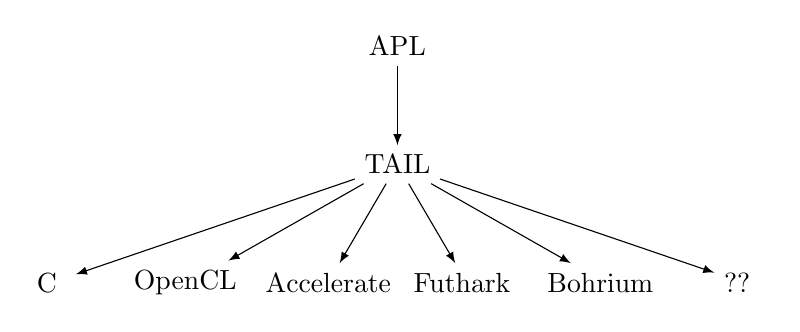
\begin{tikzpicture}[edge from parent/.style={draw,-latex},
                    sibling distance=5em,
                    every node/.style = {shape=rectangle,
                    align=center}]
  \node {APL}
    child { node {TAIL}
      child { node { C } } 
      child { node { OpenCL } } 
      child { node {Accelerate} }
      child { node { Futhark } } 
      child { node { Bohrium } } 
      child { node { ?? } } 
    };
\end{tikzpicture}

\end{frame}

% \begin{frame}[fragile]
% \frametitle{Why targeting Accelerate? }

% \begin{itemize}
% \item Seemed like an obvious choice given the similarities with TAIL
% \item The Accelerate people had shown interest
% \item Using their segmented reductions and scans, we could potentially
%   also perform NESL-like flattening and thus allow nested computations.
% \end{itemize}

% A lot of hurdles came up, mostly because the EDSL-nature of
% Accelerate. More on that later!
% \end{frame}

% \begin{frame}[fragile]
% \frametitle{Example: TAIL $->$ Accelerate}

% \tiny
% \begin{verbatim}
% module Main where
% import qualified Prelude as P
% import Prelude ((+), (-), (*), (/))
% import Data.Array.Accelerate
% import qualified Data.Array.Accelerate.CUDA as Backend
% import qualified APLAcc.Primitives as Prim
 
% program :: Acc (Scalar P.Double)
% program
%   = let v0 = Prim.iotaV 100 :: Acc (Array DIM1 P.Int) in
%       let v3
%             = Prim.consV (constant (0 :: P.Int)) v0 :: Acc (Array DIM1 P.Int)
%         in
%         Prim.reduce (+) (constant (0.0 :: P.Double))
%           (Prim.each (\ v11 -> P.max (constant (-50.0 :: P.Double)) v11)
%              (Prim.each (\ v10 -> P.min (constant (50.0 :: P.Double)) v10)
%                 (Prim.each (\ v9 -> constant (50.0 :: P.Double) * v9)
%                    (Prim.zipWith (/)
%                       (Prim.each Prim.i2d
%                          (Prim.drop (constant (1 :: P.Int))
%                             (Prim.zipWith (-) v3
%                                (Prim.transp
%                                   (Prim.rotateV (constant (-1 :: P.Int)) (Prim.transp v3))))))
%                       (Prim.eachV (\ v2 -> constant (1.0e-2 :: P.Double) + v2)
%                          (Prim.eachV Prim.i2d v0))))))
% main = P.print (Backend.run program)
% \end{verbatim}

% \end{frame}

\begin{frame}
\frametitle{Benchmarks}

\begin{tabular}{llrr}
\textbf{Benchmark} & \textbf{Problem size} & \textbf{TAIL C} & \textbf{TAIL Acc} \\
\midrule
Integral       & N = 10,000,000 &  46.90 &    3.10 \\
Signal         & N = 50,000,000 & 209.03 &   16.1  \\
Game-of-Life   & $40\times 40$, N = 2,000 &  28.70 & 2.30 \\
Easter         & N = 3,000 &   33.96 &         -  \\
Black-Scholes  & N = 10,000&    54.0 &      -     \\
Sobol MC $\pi$ & N = 10,000,000  & 4881.30  &   2430.30   \\
HotSpot        & $1024\times 1024$, N = 360 &    6072.93 &   2.03
\end{tabular}

\vspace{1cm}

\begin{itemize}
\item Timings in milliseconds. Averages over 30 executions.
\end{itemize}

\end{frame}


% \begin{frame}
% \frametitle{Difficulties using Accelerate}

% (I might be too honest here!)

% \begin{itemize}
% \item No easy to target AST-representation (yet) and generating
%   Haskell code is not ideal
% \item Shapes in Accelerate have the outer-most dimension placed
%   innermost in the the Shape-list. Making certain operations difficult
%   to implement efficiently (e.g. vertical rotation)
% \item When using Accelerate looping constructs (e.g. \texttt{awhile})
%   it seems that sharing is not recovered (e.g. let bound variables
%   outside the loop are inlined, into the loop)
% \item No real cost-model. We are unable to reason about memory layout
%   (e.g. after a transposition).
% \item No control over memory allocations
% \item Hard to debug
% \item Hard to benchmark% . You have to use various tricks to force a
%   % computation, and avoid including time spent by calling \texttt{nvcc}.
% \item No mutable array updates
% \end{itemize}

% \end{frame}

% \begin{frame}
% \frametitle{What I'm working on while at Chalmers}

% ~APL \\
% $\quad\Downarrow$ \\
% ~TAIL $\quad\Rightarrow\quad$Accelerate \\
% $\quad\Downarrow$\\
% ~~\ldots \\
% $\quad\Downarrow$ \\
% ~~\ldots \\
% $\quad\Downarrow$ \\
% \fbox{Some new functional low-level GPU intermediate language} \\
% $\quad\Downarrow$ \\
% OpenCL/CUDA
% \end{frame}

% %------------------------------------------------

% \begin{frame}
% \frametitle{Requirements}
% \begin{itemize}
% % \item Interpreted environment (e.g. APL, MATLAB, NumPy, R)
% %   \begin{itemize}
% %   \item implies dynamic compilation (JIT)
% %   \item implies dynamic garbage collection
% %   \end{itemize}

% \item Ability to optimise
%   \begin{itemize}
%   \item Consistent cost-model
%   \item Control over memory allocations
%   \item Control over when fusion/materialization occurs
%   \end{itemize}
% \item (Array updates in sequential code of kernel bodies)

% % \item Optimised idioms (e.g. 100x100 identity matrix: (⍳100)∘.=(⍳100),
% %   should be represented as a sparse matrix)
% \end{itemize}
% \end{frame}

% % \begin{frame}
% %   \frametitle{Next steps}
% %   \begin{itemize}
% %   \item Frontend
% %     \begin{itemize}
% %     \item Add array indexing
% %     \item Support DNA-application from Dyalog
% %     \item Support benchmarks from various old APL-papers
% %     \end{itemize}
% %   \item Accelerate backend
% %     \begin{itemize}
% %     \item Convert TAIL shapes to Accelerate shapes correctly
% %     \item Type-checker targetting their HOAS representation
% %     \item Mersenne Twister in Accelerate
% %     \item Support more primitives
% %     \end{itemize}
% %   \end{itemize}
% % \end{frame}

% \defverbatim{\tc}{%
% \begin{verbatim}
% equal ← { ∧/,⍺=⍵ }

% pi ← { 4×(+/1>+/(?⍵ 2⍴0)*2)÷⍵ }

% tc ← { ({⍵∨⍵∨.∧⍵} ⍣ ≡) ⍵ }
% \end{verbatim}
% }

% \defverbatim{\tcanno}{%
% \begin{verbatim}
% ⍝○ equal : [a]r → [a]r → bool
% equal ← { ∧/,⍺=⍵ }

% ⍝○ pi : int → double
% pi ← { 4×(+/1>(+/(?⍵ 2⍴0)*2)*÷2)÷⍵ }

% ⍝○ [bool]2 → [bool]2
% tc ← { ({⍵∨⍵∨.∧⍵} ⍣ ≡) ⍵ }
% \end{verbatim}
% }

% \begin{frame}[fragile]
%   \frametitle{Latest addition: Type annotations in APL code}

% \only<1>{\tc}
% \only<2->{\tcanno
% Disclosure: still pretty buggy}

% \end{frame}

% \begin{frame}[fragile]
%   \frametitle{Benefits of type annotations}

%   \begin{itemize}
%   \item Easier debugging, through improved error messages
%   \item Machine checked documentation
%   \item A necessity for compiling certain programs - even
%     parsing APL is undecidable!
%   \item Will allow for introducing dependent types, with user-written
%     types. (e.g. tracking complete shape information, not just ranks)
%   \item First steps towards a module system for APL, supporting
%     separate compilation of modules.
%   \end{itemize}

% \end{frame}

\begin{frame}
\frametitle{Restrictions}
\begin{itemize}
\item No nested arrays
\item Lexical scoping (ISO APL Standard specifies dynamic scoping)
\item No efficient implementation of boolean arrays as bit-arrays
% \item No dynamic conversions between integer and doubles (APL normally
%   does this e.g. if overflow would otherwise occur)
\item Reshapes not possible when size of shape-vector is unknown
% \item Several built-ins are still missing
% \item No labels and gotos, only limited branching
% \item No recursion
\item No execute (⍎, expression evaluation)
\item (\ldots)
\end{itemize}
\end{frame}


\begin{frame}
  \frametitle{Future work on TAIL}
  \begin{itemize}
  \item Annotations for GPU vs. CPU execution
  \item Other annotations controlling code generation (not clear what
    they should be yet)
  \item Ability to drop down to a lower level (like inline assembler)
  \item Tracking complete shape information, using dependent types
    (like QUBE)
  \item Region-inference for memory management
  \item Additional primitives
  \item Integration with real APL interpreter (Dyalog)
  % \item JIT compilation
  % \item Support nested arrays (flattening or through SNESL?)
  % \item Boolean array encode/decode?
  \end{itemize}
\end{frame}

% \begin{frame}
% \frametitle{References}
% \footnotesize{
% \begin{thebibliography}{99} % Beamer does not support BibTeX so references must be inserted manually as below
% \bibitem{p1} Compiling a Subset of APL Into a Typed Intermediate Language.
% \newblock Martin Elsman and Martin Dybdal, 2014
% \newblock \emph{ARRAY'14}

% \bibitem{p1} Compiling APL to Accelerate through a Typed Array Intermediate Language
% \newblock Michael Budde, Martin Dybdal and Martin Elsman, 2014
% \newblock \emph{ARRAY'15}

% \bibitem{p1} Accelerating Haskell array codes with multicore GPUs
% \newblock MMT Chakravarty, G Keller, S Lee, TL McDonell, V Grover, 2011
% \newblock \emph{DAMP'11}

% \bibitem{p1} APEX: The APL Parallel Executor
% \newblock Robert Bernecky, 1997
% \newblock \emph{Master Thesis}

% \bibitem{p1} QUBE - Array Programming with Dependent Types
% \newblock Kai Trojahner, 2011
% \newblock \emph{Ph.D. thesis}

% \end{thebibliography}
% }
% \end{frame}

% \begin{frame}
% \Huge{\centerline{Questions?}}
% \end{frame}


%----------------------------------------------------------------------------------------
%	BEAMER EXAMPLES of column layouts and tables
%----------------------------------------------------------------------------------------

% \begin{frame}
% \frametitle{Multiple Columns}
% \begin{columns}[c] % The "c" option specifies centered vertical alignment while the "t" option is used for top vertical alignment

% \column{.45\textwidth} % Left column and width

% \column{.5\textwidth} % Right column and width

% \end{columns}
% \end{frame}

% \begin{frame}
% \frametitle{Table}
% \begin{table}
% \begin{tabular}{l l l}
% \toprule
% \textbf{Treatments} & \textbf{Response 1} & \textbf{Response 2}\\
% \midrule
% Treatment 1 & 0.0003262 & 0.562 \\
% Treatment 2 & 0.0015681 & 0.910 \\
% Treatment 3 & 0.0009271 & 0.296 \\
% \bottomrule
% \end{tabular}
% \caption{Table caption}
% \end{table}
% \end{frame}


\begin{frame}[plain,c]{}
  \centering
  Part II
  
 \huge  FCL: Hierarchical data-parallel GPU programming
\end{frame}

\tikzset{snake arrow/.style=
{-stealth,
decorate,
decoration={snake,amplitude=.4mm,segment length=2mm,post length=0.9mm}},
}

\section{CPU vs. GPU}

\begin{frame}[fragile]
\frametitle{Standard CPU}
% \only<1-3>{
% \begin{tikzpicture}
% \begin{scope}[every edge/.append style = {snake arrow}]
% \node  at (0,2.5) {\footnotesize Core 0}; 
% \node  at (1.25,2.5) {\footnotesize Core 1}; 
% \node  at (2.5,2.5) {\footnotesize Core 2}; 
% \node  at (3.75,2.5) {\footnotesize Core 3}; 
% \draw (0,2) edge (0,0)
%       (1.25,2) edge (1.25,0)
%       (2.5,2) edge (2.5,0)
%       (3.75,2) edge (3.75,0);
% \end{scope}
% \end{tikzpicture}
% }
%\only<4->
{
\begin{tikzpicture}
\begin{scope}[every edge/.append style = {snake arrow}]
\node  at (0,2.5) {\footnotesize Core 0}; 
\node  at (1.25,2.5) {\footnotesize Core 1}; 
\node  at (2.5,2.5) {\footnotesize Core 2}; 
\node  at (3.75,2.5) {\footnotesize Core 3}; 
\draw (0,1) edge (0,0)
      (0,2) edge (0,1)
      (1.25,0.66) edge (1.25,0)
      (1.25,1.33) edge (1.25,0.66)
      (1.25,2) edge (1.25,1.33)
      (2.5,2) edge (2.5,0)
      (3.75,2) edge (3.75,0);
\end{scope}
\end{tikzpicture}
}
% \only<5->
{
\begin{textblock*}{6cm}(6.5cm,2cm)
\includegraphics[width=\textwidth]{graphics/ivybridge.jpg}
\end{textblock*}
}
\vspace{3mm}
\begin{itemize}
\item One operation at a time
\item Few compute units (cores)
\item Fast at switching between tasks
\item Most transistors used for ``recalling''
\end{itemize}

\end{frame}

\begin{frame}[fragile]
\frametitle{GPU}
\begin{tikzpicture}
\begin{scope}[every edge/.append style = {snake arrow}]
\foreach \x in {0,...,16}
  \draw (0.25*\x,1) edge (0.25*\x,0);
\end{scope}
\foreach \y in {0,...,4}
  \draw [color=lightgray](0,0.2+0.2*\y) edge (4,0.2+0.2*\y);
%\draw [color=gray,thick](-0.25,-0.25) rectangle (4.25,1.25);
\end{tikzpicture}

% \vspace{2mm}
% \begin{tikzpicture}
% \begin{scope}[every edge/.append style = {snake arrow}]
% \foreach \x in {0,...,16}
%   \draw (0.25*\x,1) edge (0.25*\x,0);
% \end{scope}
% \foreach \y in {0,...,4}
%   \draw [color=lightgray](0,0.2+0.2*\y) edge (4,0.2+0.2*\y);
% %\draw [color=gray,thick](-0.25,-0.25) rectangle (4.25,1.25);
% \end{tikzpicture}

\vspace{10mm}

\begin{textblock*}{4cm}(8.2cm,1cm)
\includegraphics[width=\textwidth]{graphics/gtx980}
\end{textblock*}

\begin{itemize}
\item Identical operations on diff. data
\item Thousands of compute units (cores)
\item Tasks executed in order (queued)
\item Most transistors used for computing
\end{itemize}

\end{frame}


\begin{frame}
\frametitle{Why a new low-level language for GPU computing?}
\begin{itemize}
\item Composability and agility
  \begin{itemize}
  \item Built in fusion, user-controlled
  \end{itemize}

\item Compare programs/algorithms
  \begin{itemize}
  \item Predictability, no black box wrt. performance
  \item Ability to optimize
  \end{itemize}
\item A quest for a functional GPU language for algorithms researchers
\item Intermediate language for optimizing compilers
\end{itemize}
\end{frame}

\begin{frame}[fragile]
\frametitle{Reverse: A simple example}

\begin{verbatim}
sig reverse : [a] -> [a]
fun reverse arr =
  let n = length arr
  in generate n (fn i => index arr (n - i - 1))
\end{verbatim}

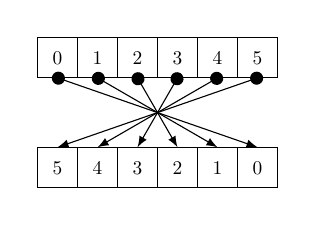
\begin{tikzpicture}[>=latex, scale=0.7, every node/.style={scale=0.7}]
\matrix[mymat, anchor=west,style={nodes=draw}]
at (0,0) 
(mat1)
{
0 & 1 & 2 & 3 & 4 & 5 \\
};
\matrix[mymat,anchor=west, style={nodes=draw}]
at (0,-2)
(mat2)
{
5 & 4 & 3 & 2 & 1 & 0 \\
};

\begin{scope}[shorten <= -2pt]
\draw[*->]
  (mat1-1-1.south) -- (mat2-1-6.north);
\draw[*->]
  (mat1-1-2.south) -- (mat2-1-5.north);
\draw[*->]
  (mat1-1-3.south) -- (mat2-1-4.north);
\draw[*->]
  (mat1-1-4.south) -- (mat2-1-3.north);
\draw[*->]
  (mat1-1-5.south) -- (mat2-1-2.north);
\draw[*->]
  (mat1-1-6.south) -- (mat2-1-1.north);
\end{scope}
\end{tikzpicture}


\pause

How is this executed on a GPU?
\begin{itemize}
\item Sequential in a single thread?
\item Performed in a single block?
\item Performed among threads in a grid?
\end{itemize}

\end{frame}

\begin{frame}[fragile]
\frametitle{Reverse: Distributed}

{\small
\begin{verbatim}
sig revBlock : [a] -> [a]<block>
fun revBlock arr = push <block> (reverse arr)

sig revDistribute : int -> [a] -> [a]<grid>
fun revDistribute chunkSize arr =
  splitUp chunkSize arr
   |> map reverseBlock
   |> reverse
   |> concat chunkSize
\end{verbatim}
}

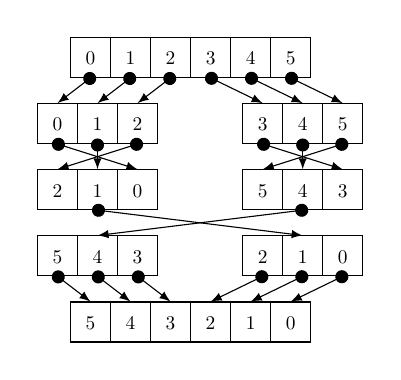
\begin{tikzpicture}[>=latex, scale=0.7, every node/.style={scale=0.7}]
\matrix[mymat, anchor=west,style={nodes=draw}]
at (0.6,0) 
(mat1)
{
0 & 1 & 2 & 3 & 4 & 5 \\
};

\matrix[mymat, anchor=west,style={nodes=draw}]
at (0,-1.2) 
(mat21)
{
0 & 1 & 2 \\
};

\matrix[mymat, anchor=west,style={nodes=draw},right of=mat21]
at (4,-1.2) 
(mat22)
{
3 & 4 & 5 \\
};

\matrix[mymat, anchor=west,style={nodes=draw}]
at (0,-2.4) 
(mat31)
{
2 & 1 & 0 \\
};

\matrix[mymat, anchor=west,style={nodes=draw},right of=mat31]
at (4,-2.4) 
(mat32)
{
5 & 4 & 3 \\
};


\matrix[mymat, anchor=west,style={nodes=draw}]
at (0,-3.6) 
(mat41)
{
5 & 4 & 3 \\
};

\matrix[mymat, anchor=west,style={nodes=draw}, right of=mat41]
at (4,-3.6) 
(mat42)
{
2 & 1 & 0 \\
};

\matrix[mymat,anchor=west, style={nodes=draw}]
at (0.6,-4.8)
(mat5)
{
5 & 4 & 3 & 2 & 1 & 0 \\
};
\begin{scope}[shorten <= -2pt]
\draw[*->]
  (mat1-1-1.south) -- (mat21-1-1.north);
\draw[*->]
  (mat1-1-2.south) -- (mat21-1-2.north);
\draw[*->]
  (mat1-1-3.south) -- (mat21-1-3.north);
\draw[*->]
  (mat1-1-4.south) -- (mat22-1-1.north);
\draw[*->]
  (mat1-1-5.south) -- (mat22-1-2.north);
\draw[*->]
  (mat1-1-6.south) -- (mat22-1-3.north);

\draw[*->]
  (mat21-1-1.south) -- (mat31-1-3.north);
\draw[*->]
  (mat21-1-2.south) -- (mat31-1-2.north);
\draw[*->]
  (mat21-1-3.south) -- (mat31-1-1.north);
\draw[*->]
  (mat22-1-1.south) -- (mat32-1-3.north);
\draw[*->]
  (mat22-1-2.south) -- (mat32-1-2.north);
\draw[*->]
  (mat22-1-3.south) -- (mat32-1-1.north);

\draw[*->]
  (mat31-1-2.south) -- (mat42-1-2.north);
\draw[*->]
  (mat32-1-2.south) -- (mat41-1-2.north);


\draw[*->]
  (mat41-1-1.south) -- (mat5-1-1.north);
\draw[*->]
  (mat41-1-2.south) -- (mat5-1-2.north);
\draw[*->]
  (mat41-1-3.south) -- (mat5-1-3.north);
\draw[*->]
  (mat42-1-1.south) -- (mat5-1-4.north);
\draw[*->]
  (mat42-1-2.south) -- (mat5-1-5.north);
\draw[*->]
  (mat42-1-3.south) -- (mat5-1-6.north);
\end{scope}
\end{tikzpicture}
\end{frame}

\begin{frame}[fragile]
  \frametitle{Reverse: Generated OpenCL}
% \begin{verbatim}
% sig revKernel : [int] -> [int]<grid>
% kernel revKernel arr = revDistribute #BlockSize arr
%   config #BlockSize = 256
% \end{verbatim}
% ~
For block size 256, FCL generates:

{\tiny
  \begin{verbatim}
__kernel void revDistribute(__global int* arrInput_0, int lenInput_1,
                            __global int* arrOutput_3) {
    int n_2 = lenInput_1 / 256;
    int blocksQ_5 = n_2 / get_num_groups(0);
    for (int i_6 = 0; i_6 < blocksQ_5; i_6++) {
        int j_8 = (get_group_id(0) * blocksQ_5) + i_6;
        arrOutput_3[((j_8 * 256) + get_local_id(0))] = 
            arrInput_0 [((((n_2 - j_8) - 1) * 256) + ((256 - get_local_id(0)) - 1))];
        barrier(CLK_LOCAL_MEM_FENCE);
    }
    if (get_group_id(0) < (n_2 % get_num_groups(0))) {
        int j_16 = (get_num_groups(0) * blocksQ_5) + get_group_id(0);
        arrOutput_3[((j_16 * 256) + get_local_id(0))] = 
            arrInput_0 [((((n_2 - j_16) - 1) * 256) + ((256 - get_local_id(0)) - 1))];
        barrier(CLK_LOCAL_MEM_FENCE);
    }
}
\end{verbatim}
}
\end{frame}

\begin{frame}[fragile,fragile]
  \frametitle{Two array types}
  \framesubtitle{(from Obsidian)}

  \begin{itemize}
  \item Pull arrays: for organizing computation, indexable no concatenation
    \begin{verbatim}
       [int], [bool], [[int]]\end{verbatim}
  \item Push arrays: for writing to memory, non indexable, supports concatenation
    \begin{verbatim}
       [int]<thread>, [int]<block>, [int]<grid>\end{verbatim}
   \item Both supporting fusion
  \end{itemize}  
\end{frame}

\begin{frame}[fragile]
  \frametitle{Array types in reverse}
\begin{verbatim}
sig revDistribute : int -> [a] -> [a]<grid>
fun revDistribute chunkSize arr =
  splitUp chunkSize arr    -- [[a]]
   |> map reverseBlock     -- [[a]<block>]
   |> reverse              -- [[a]<block>]
   |> concat chunkSize     -- [a]<grid>

sig push : <lvl> -> [a] -> [a]<lvl>
sig splitUp : int -> [a] -> [[a]]
sig concat : int -> [[a]<lvl>] -> [a]<1+lvl>
\end{verbatim}

\end{frame}

\begin{frame}[fragile]
  \frametitle{Matrix transposition}
  \framesubtitle{A basic approach}

\begin{verbatim}
sig transpose : int -> int -> [a] -> [a]
fun transpose cols rows elems =
  generate (cols * rows)
           (fn n =>
              let i = n / rows in
              let j = n % rows
              in index elems (j * rows + i))
\end{verbatim}

\end{frame}

\begin{frame}[fragile]
  \frametitle{Matrix transposition}
  \framesubtitle{Tiled}

\includegraphics[width=\textwidth]{../sharedTranspose-1024x409.jpg}

\quad(Figure by NVIDIA)
\end{frame}


\begin{frame}[fragile]
  \frametitle{Matrix transposition}
  \framesubtitle{Tiled}

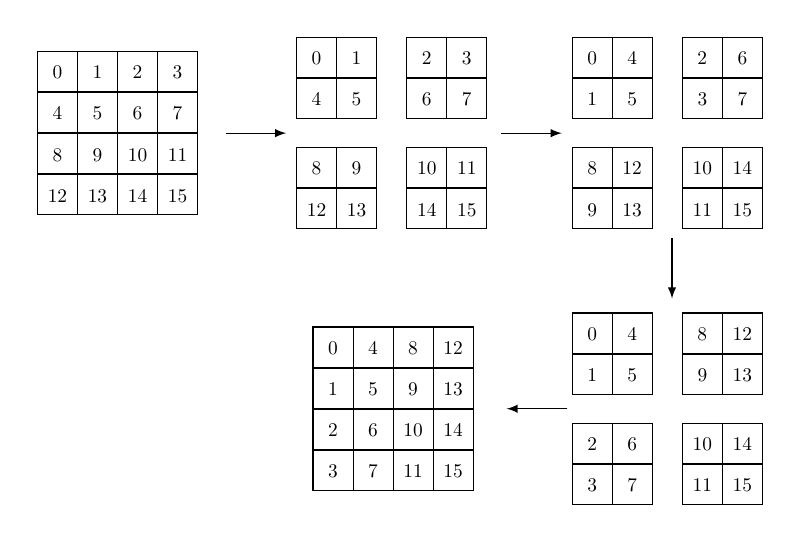
\begin{tikzpicture}[>=latex, scale=0.7, every node/.style={scale=0.7}]
\matrix[mymat, anchor=west,style={nodes=draw}]
at (0.3,0) 
(mat1)
{
0 & 1 & 2 & 3 \\
4 & 5 & 6 & 7 \\
8 & 9 & 10 & 11 \\
12 & 13 & 14 & 15 \\
};
\matrix[mymat, anchor=west,style={nodes=draw}]
at (5,1) 
(mat21)
{
0 & 1 \\
4 & 5 \\
};
\matrix[mymat, anchor=west,style={nodes=draw}]
at (7,1) 
(mat22)
{
2 & 3 \\
6 & 7 \\
};
\matrix[mymat, anchor=west,style={nodes=draw}]
at (5,-1) 
(mat23)
{
8 & 9 \\
12 & 13 \\
};
\matrix[mymat, anchor=west,style={nodes=draw}]
at (7,-1) 
(mat24)
{
10 & 11 \\
14 & 15 \\
};

\matrix[mymat, anchor=west,style={nodes=draw}]
at (10,1) 
(mat31)
{
0 & 4 \\
1 & 5 \\
};
\matrix[mymat, anchor=west,style={nodes=draw}]
at (12,1) 
(mat32)
{
2 & 6 \\
3 & 7 \\
};
\matrix[mymat, anchor=west,style={nodes=draw}]
at (10,-1) 
(mat33)
{
8 & 12 \\
9 & 13 \\
};
\matrix[mymat, anchor=west,style={nodes=draw}]
at (12,-1) 
(mat34)
{
10 & 14 \\
11 & 15 \\
};


\matrix[mymat, anchor=west,style={nodes=draw}]
at (10,-4) 
(mat41)
{
0 & 4 \\
1 & 5 \\
};
\matrix[mymat, anchor=west,style={nodes=draw}]
at (12,-4) 
(mat42)
{
8 & 12 \\
9 & 13 \\
};
\matrix[mymat, anchor=west,style={nodes=draw}]
at (10,-6) 
(mat43)
{
2 & 6 \\
3 & 7 \\
};
\matrix[mymat, anchor=west,style={nodes=draw}]
at (12,-6) 
(mat44)
{
10 & 14 \\
11 & 15 \\
};

\matrix[mymat, anchor=west,style={nodes=draw}]
at (5.3,-5) 
(mat5)
{
0 & 4 & 8 & 12 \\
1 & 5 & 9 & 13 \\
2 & 6 & 10 & 14 \\
3 & 7 & 11 & 15 \\
};

\begin{scope}[shorten <= -2pt]
\draw[->]
  (4,0) -- (5,0);
\draw[->]
  (9,0) -- (10,0);
\draw[->]
  (12,-2) -- (12,-3);
\draw[->]
  (10,-5) -- (9,-5);
\end{scope}
\end{tikzpicture}
\end{frame}



\begin{frame}[fragile,fragile]
\frametitle{Matrix transposition}
\framesubtitle{Tiled, using shared-memory}

{\small
\begin{verbatim}
sig transposeTiled : int -> int -> int -> [a] -> [a]<grid>
fun transposeTiled tileDim cols rows mat =
  let n = cols / tileDim
      m = rows / tileDim
  in split2DGrid tileDim cols n m mat
       |> map (force . push <block>)
       |> map (transpose tileDim tileDim)
       |> transpose n m
       |> map (push <block>)
       |> concat2DGrid tileDim n rows
\end{verbatim}
}

\begin{verbatim}
sig force : [a]<lvl> -> [a]
\end{verbatim}

\end{frame}

\begin{frame}
  \frametitle{Performance}
  \includegraphics[width=\textwidth]{../bandwidth}

  NVIDIA GeForce GTX 780 Ti (2880 cores, 875 Mhz, 3GB GDDR5)
  
  Peak bandwidth 254.90 GB/s (measured)
\end{frame}

\begin{frame}
  \frametitle{Highlights from formalism}

  \begin{itemize}
  \item Polymorphic type system, restricting e.g. the valid nesting of arrays
  \item Dynamic semantics, explaining mapping to threads, blocks, warps and grids
  \item Formalism informed our implementation
  \item Abstracts away from block/warp-virtualization
  \item Classic type safety properties
  \end{itemize}

\end{frame}

\begin{frame}
  \frametitle{Built-in operators}

  \begin{align*}
      \kw{lengthPull} :~& [\alpha] -> \kw{int} \\
     \kw{lengthPush} :~& \push{\alpha}{lvl} -> \kw{int} \\
     \kw{mapPull} :~& (\alpha -> \beta) -> [\alpha] -> [\beta] \\
     \kw{mapPush} :~& (\alpha -> \beta) -> \push{\alpha}{lvl} -> \push{\beta}{lvl} \\
     \\
     \kw{generate} :~& \kw{int} -> (\kw{int} -> \alpha) -> [\alpha] \\
     \kw{index} :~& [\alpha] -> \kw{int} -> \alpha \\
     \\
     \kw{push} :~& \lvl{lvl} -> [\alpha] -> \push{\alpha}{lvl} \\
     \kw{force} :~& \push{\alpha}{lvl} -> [\alpha] \\
     \kw{concat} :~& \kw{int} -> [\push{\alpha}{lvl}] -> \push{\alpha}{1+lvl} \\
     \\
     \kw{while} :~& ([\alpha] -> \kw{bool}) -> ([\alpha] -> \push{\alpha}{lvl}) -> \push{\alpha}{lvl} -> [\alpha]
%     % \kw{interleave} :~& \kw{int} -> (\kw{int} -> \kw{int} -> \kw{int}) -> [\push{\alpha}{lvl}] -> \push{\alpha}{1+lvl} \\
  \end{align*}
\end{frame}



\begin{frame}
  \frametitle{Future work on FCL}
  \begin{itemize}
  \item Generalize hierarchy and mapping \\
    {\small (e.g. ability to add layers, like multiple GPUs)}
  \item Tracking communication costs in semantics
  \item Use as back-end for our APL-compiler (TAIL)
  \item Multi-dimensional arrays
  \end{itemize}
\end{frame}

\begin{frame}
\frametitle{Summary}

\begin{itemize}
\item I argue that we need to focus on \textit{performance reasoning}
\item Nested arrays, but only non-nested arrays can be materialized.
\item Level hierarchy controls mapping to sequential/parallel loops
%\item FCL is very much work in progress
\end{itemize}

\end{frame}

% \begin{frame}
% \frametitle{References}
% \footnotesize{
% \begin{thebibliography}{99} % Beamer does not support BibTeX so references must be inserted manually as below
% \bibitem{p1} Hierarchical Data-Parallel Design-space Exploration on GPUs
% \newblock Joel Svensson, Mary Sheeran, Ryan Newton, 2016
% \newblock \emph{JFP'16}

% \bibitem{p2} Compiling a Subset of APL Into a Typed Intermediate Language.
% \newblock Martin Elsman and Martin Dybdal, 2014
% \newblock \emph{ARRAY'14}
% \end{thebibliography}
% }
% \end{frame}

\begin{frame}
\frametitle{Thank you}

Martin Dybdal \\
Ph.D. student \\
DIKU, University of Copenhagen \\
\texttt{dybber@dybber.dk} \\
%\texttt{@martindybdal}\\
~\\
FCL is available at: \url{http://github.com/dybber/fcl}
\end{frame}

% \appendix
% \backupbegin

% \begin{frame}
%   \frametitle{More future work on FCL}

%   \begin{itemize}
%   \item Manual memory-management
%   \item Sequential loops
%   \item Larger examples
%   \item Host-code generation
%   \end{itemize}
% \end{frame}

% \begin{frame}[fragile]
%   \frametitle{Reduction}
% \begin{verbatim}
% sig halve : [a] -> ([a], [a])
% sig zipWith : (a -> b -> c) -> [a] -> [b] -> [c]

% sig step : <lvl> -> (a -> a -> a) -> [a] -> [a]<lvl>
% fun step <lvl> f arr =
%   let x = halve arr
%   in push <lvl> (zipWith f (fst x) (snd x))
% \end{verbatim}

% \begin{tikzpicture}[>=latex, scale=0.7, every node/.style={scale=0.7}]
% \matrix[mymat, anchor=west,style={nodes=draw}]
% at (0,0) 
% (mat1)
% {
% 0 & 1 & 2 & 3 & 4 & 5 & 6 & 7 & 8 & 9 & 10 & 11\\
% };
% \matrix[mymat,anchor=west, style={nodes=draw}]
% at (2.45,-1.5)
% (mat2)
% {
% 0 & 1 & 2 & 3 & 4 & 5 \\
% };
% \matrix[mymat,anchor=west, style={nodes=draw}]
% at (2.45,-2.5)
% (mat3)
% {
% 6 & 7 & 8 & 9 & 10 & 11\\
% };

% \matrix[mymat,anchor=west, style={nodes=draw}]
% at (2.45,-4)
% (mat4)
% {
% 6 & 8 & 10 & 12 & 14 & 16\\
% };

% \node at (2,-2)
%   (addsymb) {\bf +};

% \begin{scope}[shorten <= -2pt]
% \draw[->]
%   (mat1.south) -- (mat2.north);
% \draw[->]
%   (mat3.south) -- (mat4.north);
% \end{scope}
% \end{tikzpicture}


% \end{frame}

% \begin{frame}[fragile]
%   \frametitle{Reduction}
%   \begin{verbatim}
% sig red : <lvl> -> (a -> a -> a) -> [a] -> [a]<lvl>
% fun red <lvl> f arr =
%   while (fn arr => 1 != lengthPull arr)
%         (step <lvl> f)
%         (step <lvl> f arr)
%   |> push <lvl>
% \end{verbatim}
% \end{frame}

% \begin{frame}[fragile]
%   \frametitle{Reduction}
%   \framesubtitle{OpenCL}

% {\tiny
% \begin{verbatim}
% __kernel void reduceAdd(__local volatile uchar* sbase,
%                         __global int* arrInput_0, int lenInput_1,
%                         __global int* arrOutput_2) {
%     int ub_3 = lenInput_1 >> 8;
%     int blocksQ_4 = ub_3 / get_num_groups(0);
%     for (int i_5 = 0; i_5 < blocksQ_4; i_5++) {
%         int j_7 = (get_group_id(0) * blocksQ_4) + i_5;
%         __local volatile int* arr_12 = (__local volatile int*) (sbase + 0);
%         arr_12[get_local_id(0)] = arrInput_0 [((j_7 * 256) + get_local_id(0))]
%                                 + arrInput_0 [((j_7 * 256) + (get_local_id(0) + 128))];
%         barrier(CLK_LOCAL_MEM_FENCE);
%         if (get_local_id(0) < 64) {
%             arr_12[get_local_id(0)] = arr_12 [get_local_id(0)] + arr_12 [(get_local_id(0) + 64)];
%         }
%         barrier(CLK_LOCAL_MEM_FENCE);
%         if (get_local_id(0) < 32) {
%             arr_12[get_local_id(0)] = arr_12 [get_local_id(0)] + arr_12 [(get_local_id(0) + 32)];
%         }
%         barrier(CLK_LOCAL_MEM_FENCE);
%         if (get_local_id(0) < 16) {
%             arr_12[get_local_id(0)] = arr_12 [get_local_id(0)] + arr_12 [(get_local_id(0) + 16)];
%         }
%         barrier(CLK_LOCAL_MEM_FENCE);
%         if (get_local_id(0) < 8) {
%             arr_12[get_local_id(0)] = arr_12 [get_local_id(0)] + arr_12 [(get_local_id(0) + 8)];
%         }
%         barrier(CLK_LOCAL_MEM_FENCE);
%         if (get_local_id(0) < 4) {
%             arr_12[get_local_id(0)] = arr_12 [get_local_id(0)] + arr_12 [(get_local_id(0) + 4)];
%         }
%         barrier(CLK_LOCAL_MEM_FENCE);
%         if (get_local_id(0) < 2) {
%             arr_12[get_local_id(0)] = arr_12 [get_local_id(0)] + arr_12 [(get_local_id(0) + 2)];
%         }
%         barrier(CLK_LOCAL_MEM_FENCE);
%         if (get_local_id(0) < 1) {
%             arr_12[get_local_id(0)] = arr_12 [get_local_id(0)] + arr_12 [(get_local_id(0) + 1)];
%         }
%         barrier(CLK_LOCAL_MEM_FENCE);
%         if (get_local_id(0) < 1) {
%             arrOutput_2[(j_7 + get_local_id(0))] = arr_12 [get_local_id(0)];
%         }
%         barrier(CLK_LOCAL_MEM_FENCE);
%     }
%     if (get_group_id(0) < (ub_3 % get_num_groups(0))) {
%         int j_36 = (get_num_groups(0) * blocksQ_4) + get_group_id(0);
%         __local volatile int* arr_41 = (__local volatile int*) (sbase + 0);
%         arr_41[get_local_id(0)] = arrInput_0 [((j_36 * 256) + get_local_id(0))] + arrInput_0 [((j_36 * 256) + (get_local_id(0) + 128))];
%         barrier(CLK_LOCAL_MEM_FENCE);
%         if (get_local_id(0) < 64) {
%             arr_41[get_local_id(0)] = arr_41 [get_local_id(0)] + arr_41 [(get_local_id(0) + 64)];
%         }
%         barrier(CLK_LOCAL_MEM_FENCE);
%         if (get_local_id(0) < 32) {
%             arr_41[get_local_id(0)] = arr_41 [get_local_id(0)] + arr_41 [(get_local_id(0) + 32)];
%         }
%         barrier(CLK_LOCAL_MEM_FENCE);
%         if (get_local_id(0) < 16) {
%             arr_41[get_local_id(0)] = arr_41 [get_local_id(0)] + arr_41 [(get_local_id(0) + 16)];
%         }
%         barrier(CLK_LOCAL_MEM_FENCE);
%         if (get_local_id(0) < 8) {
%             arr_41[get_local_id(0)] = arr_41 [get_local_id(0)] + arr_41 [(get_local_id(0) + 8)];
%         }
%         barrier(CLK_LOCAL_MEM_FENCE);
%         if (get_local_id(0) < 4) {
%             arr_41[get_local_id(0)] = arr_41 [get_local_id(0)] + arr_41 [(get_local_id(0) + 4)];
%         }
%         barrier(CLK_LOCAL_MEM_FENCE);
%         if (get_local_id(0) < 2) {
%             arr_41[get_local_id(0)] = arr_41 [get_local_id(0)] + arr_41 [(get_local_id(0) + 2)];
%         }
%         barrier(CLK_LOCAL_MEM_FENCE);
%         if (get_local_id(0) < 1) {
%             arr_41[get_local_id(0)] = arr_41 [get_local_id(0)] + arr_41 [(get_local_id(0) + 1)];
%         }
%         barrier(CLK_LOCAL_MEM_FENCE);
%         if (get_local_id(0) < 1) {
%             arrOutput_2[(j_36 + get_local_id(0))] = arr_41 [get_local_id(0)];
%         }
%         barrier(CLK_LOCAL_MEM_FENCE);
%     }
% }
% \end{verbatim}}

% \end{frame}
% \backupend


\end{document}